\chapter{Bearbeitung der Aufgaben}
\section{Koaxialkabel Simulator}\label{sec:ag3_1}

Das elektrische Verhalten eines Koaxialkabels lässt sich durch das Ersatzschaltbild \ref{koaxialkabel1} beschreiben. Hierbei stellt $R_1$ den ohmschen Längswiderstand dar, der von der Leitungslänge, dem Leitungsquerschnitt und dem Material abhängt.

Das induktive Verhalten des Kabels wird durch $L_1$ simuliert. Jeder stromdurchflossene Leiter baut ein Magnetfeld auf, die Änderung des Magnetfelds induziert eine Spannung, die dem Stromfluss entgegen wirkt und diesen abschwächt.

Durch den Isolationswert $R_2$ werden Verlustströme betrachtet, die zwischen dem inneren und äußeren Leiter des Koaxialkabels auftreten. Diese Leckströme entstehen, da es in der Realität keinen idealen Isolator gibt.

Zuletzt beinhaltet das Ersatzschaltbild noch die Leitungskapazität $C_1$. Ist am Ende der Leitung ein Verbraucher $R_f$ angeschlossen, so liegt an diesem eine Spannung an. In Folge dessen besteht auch zwischen Hin- und Rückleiter eine Potenzialgefälle. Beide Leiter verhalten sich, aufgrund der Ladungsdifferenz, somit wie die Platten eines Kondensators\footnote{Quelle: Leitungstechnik, Dipl.-Ing.(FH) Christian Wolff, 2009}. 

\begin{figure}[h]
	\centering
	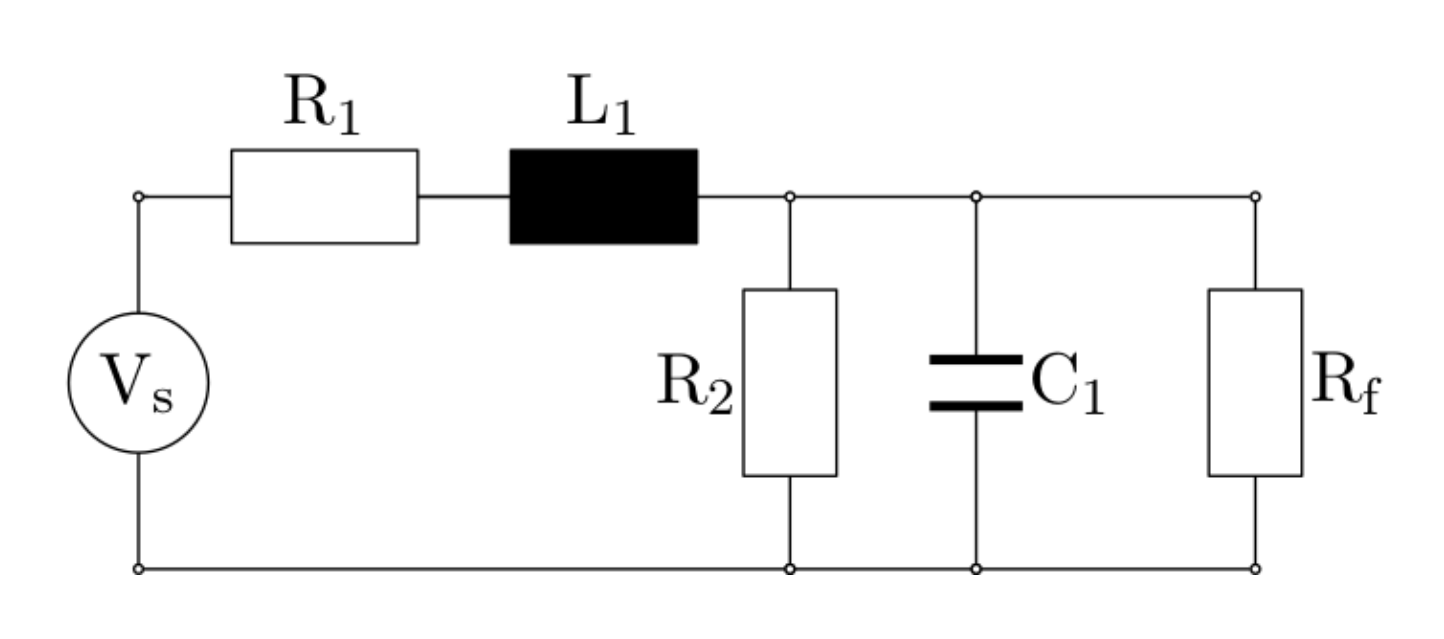
\includegraphics[width=0.7\textwidth]{data/Koaxialkabel1}
	\caption{Ersatzschaltbild Koaxialkabel}
	\label{koaxialkabel1}
\end{figure}

Mit den Routinen, die in Aufgabe 2.3 entwickelt wurden lässt sich nun dieses Segment eines Koaxialkabels simulieren. Hierzu übergibt man der Methode \texttt{calculate\_matrices} (siehe \ref{calculate_matrices}) die Netzliste \ref{netlist1}.

\begin{lstlisting}[caption={Netzliste Koaxialkabel}, label=netlist1]
Vs 1 0 12
L1 2 3 0.00025
R1 1 2 0.001
C1 3 0 0.0000001
R2 0 3 1500
Rf 0 3 1500
\end{lstlisting}

Berechnet werden nun wieder die Matrizen $\mathbf{M, K}$ und $\mathbf{r}$, die die Differenzialgleichung
\begin{equation}
\mathbf{M} \frac{\text{d}}{\text{d}t} \mathbf{x} + \mathbf{K} \mathbf{x} = \mathbf{r}
\label{matrixDGL}
\end{equation}

parametrisieren. Zuletzt wird mit der Funktion \texttt{daspk} das Gleichungssystem numerisch gelöst und die Spannung an $R_f$ gezeichnet \ref{plottKK1}. Das dazu verwendete Skript befindet sich im Anhang \ref{finalesSkript}.

\begin{figure}[h]
	\centering
	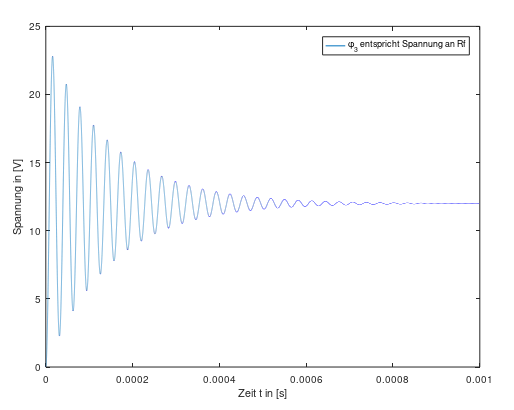
\includegraphics[width=0.7\textwidth]{data/plotKK1}
	\caption{Spannungsverlauf an Last $R_f$ bei konstanter Spannungsquelle mit 12\si{\volt}}
	\label{plottKK1}
\end{figure}

\subsubsection{Koaxialkabel mit n Gliedern}
Nun wird das RLC-Segment in \ref{koaxialkabel1} $n=10$ mal hintereinander in Reihe geschaltet (siehe \ref{koaxialkabel10}).

\begin{figure}[h]
	\centering
	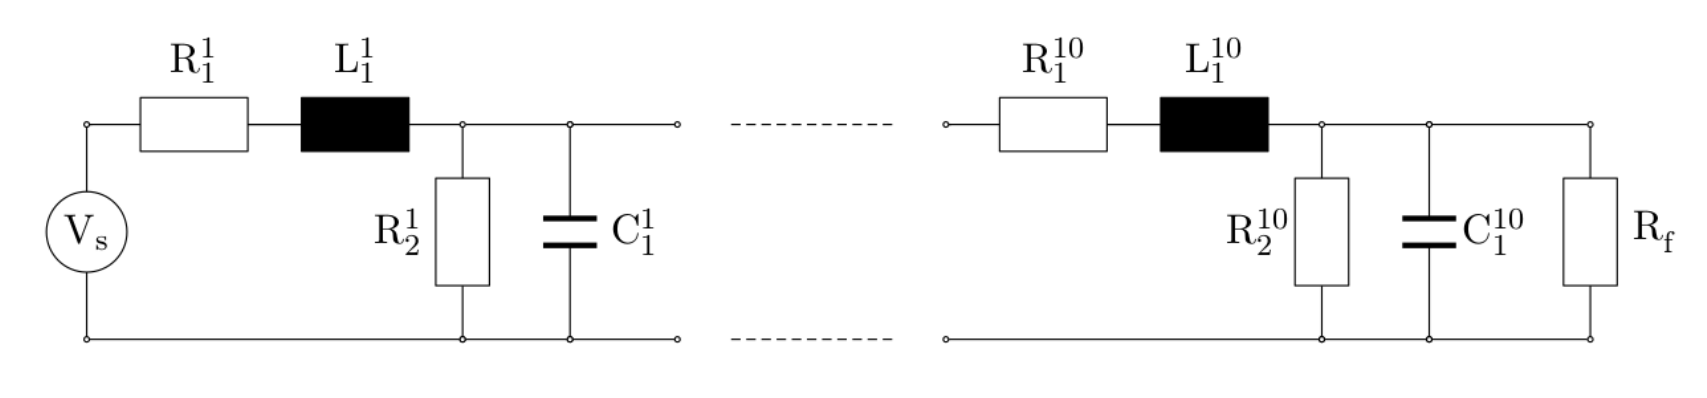
\includegraphics[width= 0.9\textwidth]{data/Koaxialkabel10}
	\caption{Ersatzschaltbild Koaxialkabel mit $n=10$ Segmenten}
	\label{koaxialkabel10}
\end{figure}

\newpage
Um zu untersuchen inwiefern diese Veränderung auf die Spannung an $R_f$ Einfluss hat, wurde ein neues Skript geschrieben, das die Unterschiede der Ausgangsspannung bei $n=1$ und $n=10$ sichtbar macht (siehe \ref{finalesSkript10}). Hierzu wurde die Netzliste für $n=10$ Segmente erstellt (siehe \ref{netlist10}), den Methoden übergeben und die Spannung an $R_f$ erneut berechnet.
Beide Ausgangsspannungen für $n=1$ und $n=10$ wurden nun in das selbe Diagramm \ref{plottKK10} eingezeichnet:

\begin{figure}[h]
	\centering
	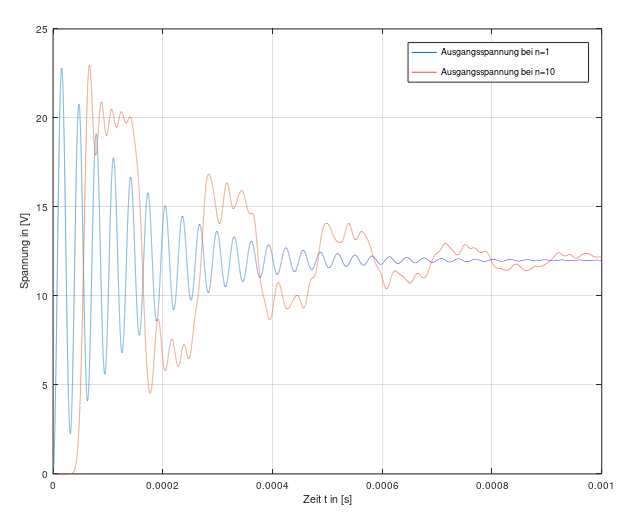
\includegraphics[width=0.75\textwidth]{data/plotKK10}
	\caption{Spannungsverlauf an Last $R_f$ für $n=1$ und $n=10$}
	\label{plottKK10}
\end{figure}

Auffällig ist zunächst einmal, dass im Fall $n=10$ das Signal durch Oberschwingungen gestört wird. Jedoch lässt sich die eigentliche Hauptschwingung dennoch gut erkennen. Bei Betrachtung dieser im Vergleich zum Fall $n=1$ wird ebenso deutlich, dass die Frequenz erheblich kleiner wurde. Ein weiterer Unterschied besteht in der Dämpfung, welche bei $n=10$ nicht so stark ist . Es dauert länger, bis die Amplitude gegen $0$ geht. Zuletzt ist noch anzumerken, dass der maximal Betrag der Spannung an $R_f$ in beiden Fällen gleich ist. Die Spannung liegt immer zwischen $0$ und $24\si{\volt}$.

Empirische Tests mit anderen Werten von $n$ ergaben, dass diese Aussagen für alle $n>1, n \in \mathbb{N}$ gelten. Folglich gilt, je mehr Segmente hinzugefügt werden, umso mehr verkleinert sich die Frequenz. Der maximale Betrag der Spannung an der Last hängt jedoch nicht von $n$ ab. Der erste Ausschlag erreicht jedes mal das maximale Niveau von knapp unter $24\si{\volt}$ und nimmt dann mit der Zeit immer weiter ab, bis die Spannung gegen $12\si{\volt}$ konvergiert.